\label{ch:impl}
This chapter presents the proposed implementation of the AHB system generator. Sec.~\ref{sec:hardover} provides an overview of the hardware described at the RTL. Sec.~\ref{sec:syslev} discusses how the ESL description is adapted to represent the hardware architecture. The challenges in creating a sound abstraction
of the hardware are elaborated. This is followed by an overview of the simulation models on both levels in Sec.~\ref{sec:sim}. A description of the hardware generator is given in Sec.~\ref{sec:generator} The chapter is ended with Sec.~\ref{sec:results} where results of property checking and simulation times are presented.

\newpage
\section{Hardware overview}
\label{sec:hardover}
\begin{figure}[hbt]
    \begin{center}
        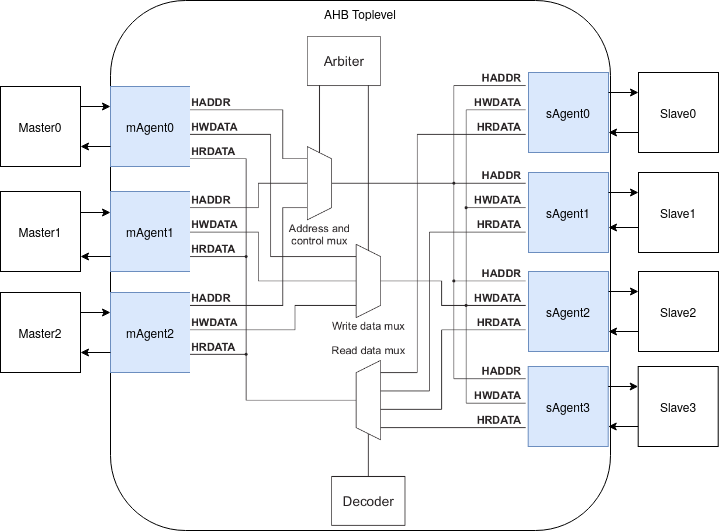
\includegraphics[width=0.8\textwidth]{figs/hw/Hw_toplevel.png}
    \end{center}
    \caption{Hardware top-level with 3 masters and 4 slaves connected}
    \label{fig:hw_toplev}
\end{figure}

For the purpose of this work, it makes little sense trying to implement the AMBA-AHB protocol from scratch starting at the ESL. It would take too much time to design the system and verify that it complies with the protocol. Instead, a trusted existing open source architecture is used. It is trusted in the sense that
it is often referenced online when "the how" of protocol implementation is inquired. Furthermore, it has been available for scrutiny online for the last 15 years.  


\subsection{Existing hardware}
\label{sub:exist}
The existing hardware is taken from the \textit{ahb\_system\_generator} found at \\
 www.opencores.com \cite{ahbsys}. This architecture is already structured for the means of generation and is implemented in VHDL, although is doesn't support wide data bus configurations it is the ideal candidate for this work. The master and slave agents was not taken from this source, they were rather redesigned to match SystemC-PPA compliant modules. This architecture supports fixed-priority, round robin and random priority arbitration. There are also modified versions of these arbitrations, where a grant is kept as long as \textbf{HBUSREQx} is asserted. The chosen arbitration for this work is the modified fixed-priority. The possibility of starvation is a drawback, but it is far less complicated to model at the ESL than for example round robin. Due to limited time, burst, split and retry transfers are not implemented in the agents. The modified extension to fixed-priority is selected to simplify an implementation of burst transfers. A study of this is presented in Sec.~\ref{sub:burstdemo}. The hardware is represented in Fig.~\ref{fig:hw_toplev} as the arbiter, decoder and wires connecting the agents. For simplicity it will collectively be referred to as the bus matrix. \par 
For reasons discussed in Sec.~\ref{sec:syslev} a property set was manually described to discover a suitable abstraction of this hardware. In the process it was
discovered that the default slave did not provide a zero cycle OKAY response when it was supposed to. It did however, provide the two cycle ERROR response as 
required by the protocol. This did not change any functionality of the design, and would never show up in simulation unless a master or agent was sensitive to this. The correct zero cycle okay response was added to simplify the completeness proof. 

   
\subsection{Master agent}
\begin{wrapfigure}[12]{l}{5cm}
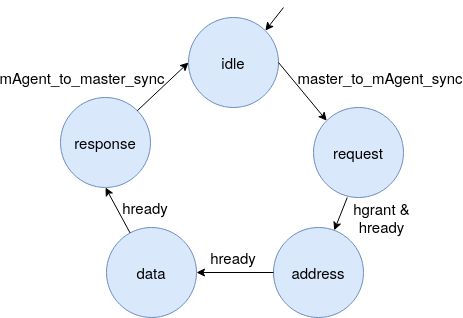
\includegraphics[width=5cm]{figs/hw/mAgent_FSM.png}
\caption{Master agent FSM}\label{fig:rafsm}
\end{wrapfigure}  

The master agent implements the master side of the AHB protocol. It is initialized to the \textit{from\_master} state, where it awaits a payload. The $agent\leftrightarrow master$ interface implements the four phase handshake in both directions. In other words, it is blocked pending a synchronization signal from the master. The payload represents only a subset of the AHB master interface. The remaining signals are hardwired to default values. \textbf{HTRANS} is an exception, this signal is controlled by the agent throughout the transfer. In an ESL description it is sometimes beneficial to use enums to represent certain encodings and signals. This is to enhance readability for the designer. These enums have been directly transferred to the RTL description. The entire payload is listed in table \ref{tab:mpayload}, where unchanged signals are marked with a dash.  

\begin{table}[hbt] 
  \label{tab:mpayload}
  \begin{tabular}{|p{25mm}|r|p{10cm}|} 
  \hline
  \textbf{Signal} & \textbf{Type} & \textbf{Content} \\
    \hline
  \textbf{HADDR} & - & - \\
    \hline
  \textbf{HWDATA} & - & - \\
    \hline
  \textbf{HWRITE} & enum & AHB\_READ, AHB\_WRITE \\
    \hline  
\textbf{HSIZE} & enum & MT\_B (byte), MT\_H (halfword), MT\_W (word) \\
    \hline
  \end{tabular}
\caption{Master out payload}
\end{table}

The return payloads consists of only \textbf{HRDATA} and \textbf{HRESP}. A key drawback that is obvious from the FSM is that the agent will return a payload 
to the master regardless of transfer direction. Surely throughput would be higher if the agent bypassed this state in the case of a write. If the transfer
status is not reported back to the master, any error would only be known locally in the agent. It would be possible to assert an error signal that is checked 
before starting a new transfer. However, any predesigned code for a CPU using the AHB protocol i.e linux, is likely to expect the error to apply to the current transfer, not the previous. To avoid limiting the bus to systems with manually tailored code, a payload is returned to the master in any case. This comes
at the cost of latency, but as discussed this is a reasonable trade-off. \par
An overview of a transfer is provided with respect to the FSM.
\begin{enumerate}
 \item \textit{from\_master}: Initial/idle state, when a synchronization signal is received, the payload is translated to pure bit and bit vector values and written to the AHB interface.
 \item \textit{Request}: \textbf{HBUSREQx} remains asserted until agent is granted the bus and the bus is ready.
 \item \textit{Address}: \textbf{HTRANS} is encoded with NONSEQ, signalling the start of a transfer. This remains encoded until the bus is ready.
 \item \textit{Data}: When the bus is ready, return payload is read from the AHB interface and written to the master.
 \item \textit{to\_master}: Agent waits for a synchronization signal from the master. The master should already be asserting its synchronization signal, but this is not a requirement.   
\end{enumerate}

The sequence of operations above does not seem to match the sequence in the protocol covered in Sec.~\ref{sec:ahb} in the previous chapter. It is, however, 
understood that address/control and data can have arbitrary values outside their respective phases, as long as the intended values are present in their 
respective phases. It is therefore also not an issue that they have the intended values outside the respective phases as well. This is provided that \textbf{HTRANS} have the correct encoding at all times. 
\newpage 

\subsection{Slave agent}
\begin{wrapfigure}[14]{l}{5.5cm}
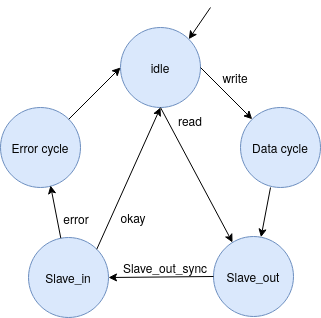
\includegraphics[width=5.5cm]{figs/hw/sAgent_FSM.png}
\caption{Slave agent FSM}\label{fig:rsfsm}
\end{wrapfigure}  

The slave agent implements the slave side of the protocol. The transitions in the FSM of Fig.~\ref{fig:rsfsm} have been simplified to make the diagram more readable. When the slave agent is selected and the start of a transfer is detected it samples the address and control signals. An additional data cycle is
required to sample the data in the case of a write transfer. The transfer payload is written out on the slave out port and the slave processes the request. The slave responds with status, and data in the case of a read. If the status is error the slave agent inserts an error cycle to provide the two cycle error response. \par
The slave agent drives \textbf{HREADY} low in all states except idle. This extends the data phase of the transfer and gives the slave time to process the request. There are no formal restrictions on the amount of wait states that can be inserted, but a total of 16 should not be exceeded for more accurate performance analysis. \par
In addition to the slave ports implementing a four phase handshake, two additional features are added to assist the system level description. The slave base address is subtracted before writing the address out to the slave. The slave only knows of its own address range starting from zero. The second feature is that the return data is zeroed after it has been sampled. The reason for this is related to the generated properties. \par
The output \textbf{HRDATA} to each master is assigned a value in each property. This can either be an updated value or the previous value. In either case, it is the \textbf{HADDR} of the granted master that determine which slave has its \textbf{HRDATA} broadcast on the response data bus. Instead of always keeping track of \textbf{HADDR}, it is easier to zero this value, when it is not valid. Why \textbf{HRDATA} is not only valid if a notify is set becomes clear when discussing the master agent interface in Sec.~\ref{sec:syslev}.   
\newpage

\section{System level representation}
\label{sec:syslev}
\begin{figure}[hbt]
    \begin{center}
        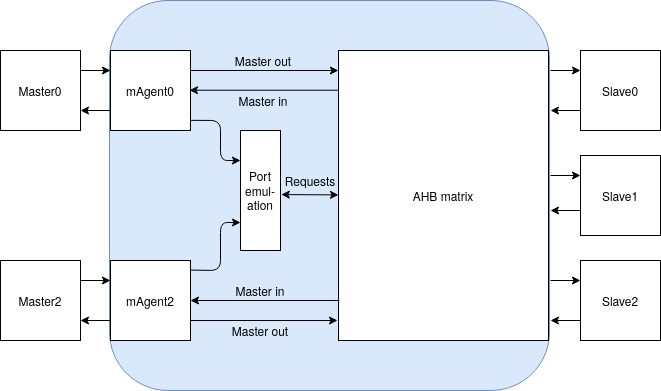
\includegraphics[width=0.8\textwidth]{figs/ESL/Syslev.png}
    \end{center}
    \caption{ESL top-level with 2 masters and 3 slaves connected}
    \label{fig:esl_toplev}
\end{figure}

When representing the AHB system at the ESL, abstraction is a priority. Ideally there would be a single SystemC-PPA describing the entire system. It is on 
the other hand not possible to represent this multi-master design without separating the master agents into their own SystemC-PPA. The reason for this is 
parallelism, and a single thread's lack of capability to represent it. Regardless of which conceptual state the system is in, any idle master can receive 
a message and proceed to request. This operation requires the output \textit{master\_to\_mAgent(x)\_notify} to be de-asserted. In addition, knowledge of this request and the message must be stored for use in a later conceptual state. This is not practical to represent at the in a single SystemC-PPA, if it is even possible. \par
Considering that the ESL needs to represent a relatively complex existing RTL description, it is necessary to manually write the properties bottom-up to get an idea of how the system level description of the bus matrix must be formed.

\subsection{Manual property set}
During the development of the initial property set it became clear that to determine the state of the bus, knowledge of past behavior is required. It is not possible to determine every state of the bus by observing internal registers of the design alone. There are registers storing which master owns the address and data bus, but this provides no information on the state of the bus when the owner is the default master. A solution is to look at past values of the transfer  control signals, but knowing how far back to look would require a fixed amount of wait states. Another much simpler alternative is to exploit that master agents are verified in separate clusters. The state of the master agents are determined as outputs to their clusters and as inputs to the bus matrix cluster. The state of the bus is now possible to determine at any time by observing the states of the master agents. \par
For all the completeness checks introduced in Sec.~\ref{sub:cipc} to hold, certain attributes must be captured in the properties. 
\begin{enumerate}
 \item The handling of requests must be captured, which happens at any time \textbf{HREADY} is driven high. In this implementation this is when the system is idle, in the address phase of a transfer and at the end of the data phase of a transfer.
 \item The transfer of a message from the master agent interface to the slave interface must be captured by representing it in visible registers. The address and data bus are not ideal candidates for physical registers to map these visible registers to. They are outputs of multiplexers, which are not updated on a clock edge. This is problematic to represent using SystemC-PPA. It is always true that when there is a request at time $t$, the message of the granted master from time $t$ is visible on the bus at time $t+1$. However, when one master loses its grant it is the default masters message that is visible on the bus. This could be either the message from $t$ or a message from $t+1$.  
 \item The signals which are outputs to the master agent interface must be determined for all masters. It is not strictly necessary to determine response data unless a slave is responding and \textbf{HREADY} is set. The transfer status is similar, except it should be determined in both cycles of a two cycle error response. \textbf{HREADY} must always be determined, and when it is high so does \textbf{HGRANTx}. Like the address and data bus, \textbf{HGRANTx} is not updated on a clock edge. This is a larger issue in this case. It is not possible to determine this signal at any other than the current time-point. The value must either be determined at time $t$, which is not possible at the ESL, or it has to be determined as the output of a function. 
\end{enumerate} 

A property set which covered all inputs and outputs was manually designed, and all completeness checks held. This property set was used as a starting point to devlop the ESL description.  

\subsection{Forming the ESL}
How to represent the interface between the master agents and the bus matrix at the ESL required much thought and experimentation. Not only must address, control and data signals reach their target, but the generated properties must hold on the design and prove completeness. A pure interface using existing SystemC-PPA ports was explored: 
\begin{itemize}
  \item \textit{Shared port}: This port enables a straight forward implementation of the interface, all signals are represented in their pure form in both directions. Implementing the correct control flow between the master agents and the bus matrix proved to be problematic. Regardless, with this interface alone
\textbf{HGRANTx} would need to be represented using actual values which as discussed is not feasible, because it is not updated on a clock edge.  
 \item \textit{Master/slave port}: Because of the rules the slave side of this interface imposes, introduced in Sec.~\ref{sub:ports}, this would merely be a more tedious implementation of the shared port. The master agent does not communicate directly with the slave. If the bus matrix was a slave it would need to write every port in order, in every cycle. This is not practical when abstraction is the goal. 
 \item \textit{Blocking port}: This port is ideal for modeling signals which control the transitions between states. Particularly the signals \textbf{HBUSREQx}, 
\textbf{HREADY} and \textbf{HGRANTx}. The master agent can signal a request with the event notify of the port, and will wait for the synchronization from the other end. This synchronization signal represents grant/ready. A second port can be used similarly to represent ready in the two phases of the transfer. The generated properties are easy to refine on the master agent. The same does not apply for the bus matrix, because each port imply an important state. In terms of properties it is only allowed to be in one of these states at a time. In reality requests for one master is handled in the same cycle as \textbf{HREADY} advances the state one or two others.  
\end{itemize}

A solution to the blocking port problem is proposed by combining all signals into a single port, which needs to represent \textbf{HBUSREQx}, \textbf{HREADY} and \textbf{HGRANTx}. This port type has been emulated using existing SystemC-PPA ports. On the master side there are two blocking out ports \textit{mAgent\_request} and \textit{bus\_ready}. On the bus matrix side there is one blocking out port \textit{update\_requests} and a shared in port \textit{requests\_in}. The emulated
port resides in its own module, but is not intended to be counted as its own SystemC-PPA, rather it is treated in this implementation as if it was a regular
port. \par
The port waits for a synchronization signal from \textit{update\_requests}. When it is received it peeks on all master agents request inputs and writes out a compound with this information to the \textit{requests\_in} port. The port decides internally which master has the highest priority, and performs a non-blocking read from its request port. This is followed by the port performing a non-blocking read of any \textit{bus\_ready} port which has an agent waiting. 
By only performing a non blocking read when an agent is waiting ensures that the wait function is not called before the port is again blocked at \textit{update\_requests}. This way accurate simulation is accomplished together with a usable property set. \par

\subsubsection{Master agent}
\begin{wrapfigure}{l}{5.5cm}
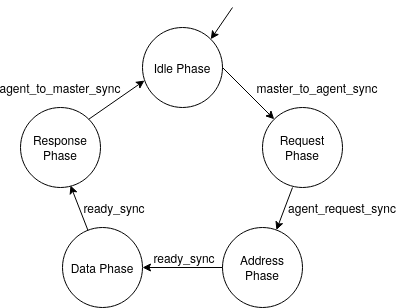
\includegraphics[width=5.5cm]{figs/ESL/mAgent_ESL.png}
\caption{master agent FSM}\label{fig:eafsm}
\end{wrapfigure}

The master agent reads a payload from its master from a blocking\_in port. When received,  the payload is added together with other control signals to a compound that represents the ahb master out interface. This compound is written to the bus on a shared\_out port. A shared port is used for two reasons: The interface output signals must be determined in the properties throughout the entire transfer. This is not accomplished with a blocking port. The control signal \textbf{HTRANS} must also be updated during the transfer. The bus request is represented separately by a blocking\_out port, as described earlier. The agent proceeds through the FSM as shown in figure \ref{fig:eafsm}. When the bus is ready in the data state it reads the status and data from a shared\_in port and writes it out to its master through a blocking port. \WKSAY{The payload is written to the matrix as the state progresses to the request state because the matrix requires the payload on the address bus at $t+1$ to be fetched from the agent at time $t$. This is a misrepresentation of the protocol and there is no way around it. But it may be weird to write about this here rather than in a summary or appendix} 

\subsubsection{Bus matrix}
\begin{wrapfigure}[17]{l}{5.5cm}
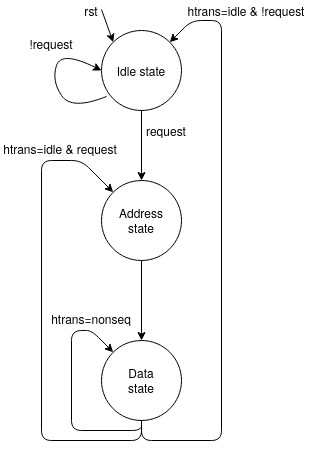
\includegraphics[width=5.5cm]{figs/ESL/Bus_fsm_new.png}
\caption{Bus matrix FSM}\label{fig:busfsm}
\end{wrapfigure}

The bus matrix is represented at the ESL with three explicit states. These three states represent the transfer phases only when the transitions $Address\rightarrow Data$ are followed. This is not always the case so it is useful to distinguish the difference between the phases of the transfer and the states of the bus. If the bus is in the state $Address$, there is only one transfer in question and it is in the address phase. If the bus is in the state $Data$, there is one master with its transfer in the data phase, but there may also be a master with its transfer in its address phase. For this reason the word \textit{state} can not be used interchangeably with \textit{phase}, as they could within the master agents. \\
The communication over the emulated port type is done once in all three states as follows: \\
\begin{lstlisting}
update_request->try_write(true, sync, "state name");
requests_in->get(reqs);
mAgent_to_bus0->get(payload0); // separate shared_in ports 
mAgent_to_bus1->get(payload1); // alongside the emulated port
           .
           .
mAgent_to_bus14->get(payload14)
\end{lstlisting}   

The payload of the highest priority requesting master is stored in a struct named $AS\_regs$. This struct represents important signals on the address bus, or rather the important signals on the master interface of the master whose transfer is in the address phase. As the state transitions from $Address\rightarrow Data$ this struct is copied to another struct conveniently named $DS\_regs$. If it is a write transfer \textbf{HWDATA} is fetched from the interface of the data bus owner and stored in $DS\_regs$. This struct represents the master payload and is written out to the selected slave through a blocking\_out port. The bus matrix waits for a response from the slave which is written to all master agents through shared\_out ports. The choice to use shared ports for response data and status results in less than ideal generated properties, for it is necessary to determine these signals in all stages. For this reason they are zeroed when unimportant. The alternative is to return response data as a payload over the emulated port. This was decided against to keep this port minimal, since the port is not a proven built in interface. \textbf{HREADY} and \textbf{HGRANTx} is as mentioned part of the emulated port. \textbf{HGRANTx} is also added to the shared\_out. \textbf{HGRANTx} need to be determined through a function. This is accomplished by representing them with enums, which are later refined as function outputs in the properties. \par 
An important state is inserted to capture the first cycle in the two cycle error response, if an error occurs. This cycle is not abstracted away to successfully determine \textbf{HRESP} in the first cycle. This is an important signal according to protocol, and is therefore accounted for throughout the two cycle response. A state is inserted at the beginning of the data state in a similar manner in the case of a write transfer. Rather than abstracting away the data cycle, it is beneficial that the properties reflect that the data was sampled in the data phase rather than the address phase. Otherwise the system becomes dependent on its own limitations, which is not ideal for future improvements. \par
Various implementations of the ESL was experimented with to see which level of abstraction is the most practical. The goal is to achieve the highest possible level of abstraction. At the same time it is beneficial not to make the system dependent on its own limitations, by misrepresenting the protocol in the generated properties. The different levels of abstraction reflect the AHB protocol to a varying degree, but all have about the same simulation performance. The difference in performance is most notable in the proof time of the properties. The current implementation is considered to have the best balance between proof time and protocol representation. \WKSAY{Perhaps this last part belongs in a summary}      


\subsubsection{Properties, and signal macros}
\WKSAY{Maybe i should start with, what is a macro and what it means to refine it. Or this should be covered in chapter 2 and referred to here}
To abide by the guidelines for verification of multiple clusters introduced in Sec.~\ref{sub:clust} all communication I/O signals are refined using the common
top level signals. However, the refinement of the macros representing the emulated port require some explanation. The macro refinement on both sides will be explained in parallel. 
\begin{itemize}
 \item \textit{mAgent\_request\_notify}: Simply refined to represent \textbf{HBUSREQx} in the master agent.
 \item \textit{Update\_requests\_sync}: Refined to represent all \textbf{HBUSREQx} "or'ed" together in the bus matrix. This enables the trigger in all properties related to this port. It can also be refined to true, it is simply a matter of which properties become vacuous. The current choice is however more true to its intended use. This signal is not sufficient as assumption in the completeness description to represent all \textbf{HBUSREQx}.
 \item \textit{requests\_in}: A separate macro is generated for each request signals, all refined to their respective \textbf{HBUSREQx} in the bus matrix. These signals are sufficient to use as assumption in the completeness description.  
 \item \textit{bus\_ready\_sync}: Refined to \textbf{HREADY} in the master agent. 
 \item \textit{mAgent\_request\_sync}: Refined as \textbf{HREADY} "and'ed" with \textbf{HGRANTx} in the master agent. It is sufficient to use as assumption in the completeness description to represent \textbf{HRGRANTx}. The agent does not care about grant unless the bus is ready. 
\end{itemize} 

The final macro is best explained using a code example:\\
\begin{lstlisting}
update_requests_notify : boolean := 
  bus_to_mAgent0.hready and bus_to_mAgent1.hready or
  
  bus_to_mAgent0.hready and bus_to_mAgent0.hgrant or
  bus_to_mAgent1.hready and bus_to_mAgent1.hgrant
end macro;
\end{lstlisting}

\WKSAY{AS\_regs are refined to represent the address bus if any agent is in the address phase, DS_regs are optimized to represent data on the data bus in the data cycle, and previous values on AS_regs, or default values. States are optimized so that only default master state, address and data owner are used. \\ need to talk about vacuous properties for 1 and 2 masters. Some need to remain for the case split test to hold. In some cases they hold but witness is uncreachable}

This macro is sufficient to determine \textbf{HREADY} as an output in the completeness check because of an added assertion that proves that all readies
are equal. It is not sufficient to determine \textbf{HGRANTx} as output due to it being "and'ed" with a signal which often has opposite value. It is still added this way to provide consistency with the macro refinements in the master agent. \par
Another signal which require some explanation is \textbf{HGRANTx}. As the signal above is not sufficient to determine this as an output another solution is required. As mentioned earlier it must be determined using a function. At the ESL it is simply an enum with the name m(x)\_grant. The macro of this enum
is redefined as a boolean, and assigned a value using another macro which determines the current value of \textbf{HGRANTx} using a combination of inputs
and outputs. These signals are all listed as assumptions and determination requirements in the completeness description. \par
As mentioned earlier, the states of the master agents are used to determine the state of the bus matrix. It is not explicitly specified as a port signal at the
ESL. It is however set as a determination requirement in the completeness description of the master agent. This is sufficient to use it as an input to the
completeness description of the bus matrix. In the bus matrix this is a macro added by the automatic refinement. \par
The visible registers that are generated from the ESL are the signals of AS\_regs, DS\_regs and slave response, resp for short. All AS\_regs signals are refined
to represent its respective input from the master agent interface of whichever master is in its address state. If none apply they all are assigned default values. The same applies for all DS\_regs signals except it applies for any master in its data state. The exception is \textbf{HADDR}, this signal represents the output of the slave port which has its out notify set. This is to account for the address offset. The final signals, resp represent the \textbf{HRDATA} and \textbf{HRESP} of the responding slave, two cycles after its sync signal was received. This signal has default values as well. Representing the visible registers this way allow to transfer the data between properties without mapping a myriad of physical registers, greatly improving proof time. \par
The final set of refinements are the states. These are mostly represented using either the states of the masters alone, or the states of the masters together with either notify signals from slave ports or the address in DS\_regs. 


\subsection{Burst transfer demonstration} 
\label{sub:burstdemo}
This section covers a demonstration of a four beat incremental burst implemented with SystemC-PPA. For this demonstration a system with a single master and slave
is used and the address is constrained within the slave address range. Furthermore, the masters and slaves have not been developed to handle an early burst termination. For additional simplicity, the slave is constrained to always be ready to answer its agent in the same cycle. The data size is limited to 32-bit.

\subsubsection{RTL}
The RTL implementation of the four beat burst is rudimentary but it follows protocol when disregarding early burst termination. The predesigned arbiter and interconnect already support all types of burst transfer. The changes implemented in the master and slave agents are discussed.
\begin{itemize}
 \item \textit{Master side}: Register banks are added to the interface between a master and its agent. These are four 32-bit registers each, one for burst write data and a separate register bank for burst read data. The regular payload is extended to include \textbf{HBURST}. A new state is added to the state machine named \textit{addr\_data} which handle the concurrent clocking in/out of both address and data. The address is incremented as data is clocked in or out when \textbf{HREADY} is set. Separate shift registers are used for each direction to simplify property refinement. 
 \item \textit{Slave side}: The slave has a separate shift register for address, data and response data. In the case of a burst write, all data and addresses are clocked in. The last data in the burst is sampled, but the slave agent drives \textbf{HREADY} low to extend the transfer until it receives response from the slave. In the case of a burst read it drives \textbf{HREADY} low after the first address is sampled, to extend the transfer until the slave responds with the data. The slave must therefore calculate the remaining addresses internally using the control signals. When the agent receives the data it clocks in the remaining addresses as it clocks out the response data. The need to calculate the addresses internally renders the address register bank redundant in the RTL design. It is however very useful in refinement of property macros. 
\end{itemize}

The master still completes the burst if it receives an error in the middle of the burst, but the slave is unable to provide an error signal until the final cycle anyway. 


\subsubsection{SystemC-PPA and property refinement}
The emulated port is not essential for a single master/slave system. There are ways to implement the same functionality using blocking in/out ports selected
based on criteria. However, to illustrate that this burst functionality can be implemented on a multi master system, it is attempted to stay as true to the
original design as possible. The most feasible way to represent a burst transfer in either direction is by use of blocking ports. With exception of the notify, no signals on a blocking out port are determined unless notify is set. A shared output require all its signals to be determined in every property. The time shifted data and address in a burst transfer payload is problematic in the case of a shared out. Shared input ports can represent any time shifted payload without any issues.

\begin{itemize}
 \item \textit{emulated port}: The emulated port transfers the burst data between the master agent and bus matrix. Additional blocking read/write ports are added on the master agent side to handle the burst transfers. The \textit{mAgent\_request} port is reconfigured contain a burst helper payload and \textit{update\_requests} is reconfigured to contain the burst read payload. The port uses the burst helper to keep track of whether the transfer is a burst, and if so when to communicate over either burst blocking port. When the transfer is a burst read, the emulated port must forward the data from the bus matrix to the agent, which requires a write to a blocking port within the emulated port. As discussed, the emulated port must operate atomically and (non-)blocking write always calls a wait function. This is not problematic for a single master system, but for multiple masters this write would need to omit the wait function in this instance.       
 \item \textit{bus matrix}: The bus matrix uses the same input and output ports, only they have been reconfigured to handle burst payloads. In the case of a single transfer only the first data and address element is used. All other elements are zeroed, so the property macros can be zeroed under these conditions as well. In the case of a burst write all address and data elements are fetched from shared ports and written out to the slave. All transfers share the same port and conceptual state for writing out. In the case of a burst read the burst data is read from the slave in port and written directly out to the \textit{update\_requests} port. The original shared out port for \textbf{HRDATA} and \textbf{HRESP}is updated as well. The burst read uses separate conceptual states for both ports. The separation of the read port is necessary to determine if it was a burst read or not. The separation of \textit{update\_requests} was also necessary to remove the compound as a visible register in the generated properties. 
 \item \textit{master agent}: When the master agent receives a request it also reads a shared in port which contains possible burst data. This data, along with
the base address, whether it is a burst and transfer direction is written out using a burst helper compound on the \textit{mAgent\_request} port. This is the actual transfer of the data at the ESL, but does not represent the transfer of data in the properties. The write to the burst port represent the burst transfer in the properties. This transfer must end in the final stage of the transfer, meaning all addresses are clocked out and the last data is valid on the bus. The synchronization signal of this port signals the data phase is over. It is simply too late to exclusively transfer the data here at the ESL.   
\end{itemize}     

To illustrate how the properties are refined to capture the transfer, some pseudo code examples will be used. The first example covers the data in a burst write from the master agent. In the RTL description the data is clocked out of a shift register to \textbf{HWDATA} output. This sequence is captured in the properties as one operation, all ending at time \textit{t\_end} as follows.
\begin{lstlisting}
for timepoints: t_end = t+4
 assume:
  at t: address_phase;
  at t: hburst = 4beat_incremental; 
  at t: hwrite = write;

 prove:
   at t_end: data_phase;
   at t_end: burst_out_hwdata0 := shiftregister_hwdata0_at_t; 
   at t_end: burst_out_hwdata1 := shiftregister_hwdata1_at_t; 
   at t_end: burst_out_hwdata2 := shiftregister_hwdata2_at_t;
   at t_end: burst_out_hwdata3 := shiftregister_hwdata3_at_t;
\end{lstlisting}

The data sequential transfer of data is represented by refining the macro definitions of \textit{burst\_out} to represent \textbf{HWDATA} at various degrees
of time shifts. 
 
\begin{lstlisting}
burst_out_hwdata0 : unsigned := prev(mAgent_to_bus0.hwdata, 3) 
burst_out_hwdata1 : unsigned := prev(mAgent_to_bus0.hwdata, 2) 
burst_out_hwdata2 : unsigned := prev(mAgent_to_bus0.hwdata)
burst_out_hwdata3 : unsigned := mAgent_to_bus0.hwdata 
\end{lstlisting}

All other important outputs can be added to the burst compound so all important outputs are determined. The state of the master agents are declared as outputs
in the completeness description in the original design. The state \textit{addr\_data} needs to be represented in the burst compound. 
\WKSAY{I need to write more about burst. address and request wait witness in master agent is unreachable because it is only one master. slave wait constraint is not necessary at all. timepoints will be fixed for all cases of burst. Need to mention the signal used as condition for the burst read state in master agent.}


\section{Simulation}
\label{sec:sim}
Simulation models carrying out the same operations are designed for both abstraction layers. One of the main benefits of modeling hardware at the ESL is simulation speed, so a time comparison is carried out between the two layers. Designing two corresponding simulation models also offers some verification. 
The aim of PDD is to do away with RTL simulation altogether, but when the ESL description is modeled after an existing hardware architecture it makes sense
to ensure that the two simulation models behave equally. \par
Master and slave dummies are connected to the bus matrix. The dummies perform simple operations to maintain a good overview of the operations. 
The master dummy alternates between single read and writes. It increments the address by 10 every transaction, and the data by 1 every write. 
The simulation lasts for the duration of $10^6$ transfers, during which the address wraps around to 0 if it reaches the end of the slave address range. \par
Assertions are used to control that data is transmitted between the intended dummies. The slave dummy has no information about which master it is operated by. 
All masters can act independently from each other, and due to the arbitration it is not so simple to monitor from a top level perspective. It is an error prone
process and it is avoided. Instead, slaves also store their response in a map. The master asserts that the slave it intended to operate is the one that responds. VHDL offer no such high level functions for monitoring, so it is difficult to assert if the payload reaches its target from a top level perspective.
\WKSAY{Im going to need to look more into this}
Accessing the default slave does not increment the transfer count, so choosing a non continuous address range will affect the simulation time.  

\subsection{Starvation}
One drawback of fixed-priority arbitration is that lower priority masters may never be granted access to the bus. When this occur depends on the amount of masters, the rate of transfer for each master and the duration of each transfer. It can be observed from RTL simulation that a fourth master is never granted access if all three higher priority masters request the bus as rapidly as allowed by
the implementation. It is not possible for an untimed ESL simulation to exactly reflect such time dependent behavior. What is important to accurately reflect in the ESL simulation is whether a master starves forever or not. \par
In the provided test bench this is modeled accurately because it is easy to observe the differences in the simulation types. If all masters request out of range it is the fifth master, rather than the fourth that starves forever. This is because the default slave responds faster and the delay between the agents response to a new request is at least three clock cycles. The fourth master is in this case granted the bus before the first master has time to request anew. There exists no such delay at the ESL, so the fourth master is never granted access here unless delay of $3*MIN\_WAIT\_TIME$ is added and $MIN\_WAIT\_TIME>0$. \par
It is not a real scenario that all masters request out of range forever, but it highlights an issue with untimed models and starvation. It is safe to say that a fourth and fifth master will at some point be granted access to the bus, because all masters will not always request access. When a system contains a high number of masters that request access to the bus at varying rates, a $3*MIN\_WAIT\_TIME$ delay inserted is likely not enough to ensure equivalent simulation behavior. \WKSAY{is the only option here a better arbitration protocol?}

\section{Generator}
\label{sec:generator}
The AHB system can be generated using a program implemented in C++, where the number of masters and slaves are required as input arguments. Allowed number of
masters and slaves are between 1 and 15. An ESL and RTL description, including test benches are generated followed by a set of operation properties and completeness descriptions. Two short scripts are included which enable the property and completeness check to be carried out with just one command from the
command line. 

\subsection{Hardware generator}
The generator reads a text file \textit{AddressMap.txt} which contains all the slave addresses. This has default values, but a user can configure the addresses freely. If a system has four slaves only the addresses of slave 0-3 will be read. If the address ranges are discontinuous it will affect the generated test bench's simulation time. These addresses are stored in a map, and used throughout the generation. The addresses are also converted to VHDL format and printed to a second text file together with number of masters and slaves to assist the automatic property refinement. \par
The ESL is generated using a C++ class which has the number of masters and slaves as well as an address map stored internally. The class uses this information to generate the bus matrix, top-level design and test bench. Global helper files are also generated which contain the slave address ranges and other common signals. All files are stored in the output folder of the generator. Not all files in this folder are generated, for example the master agent remains unchanged for every configuration. The generator returns with error if there are any files that do not generate successfully \par
The RTL is generated in the same way, and to simplify automatic property refinement the same interface and top-level signal names are used on both levels.
After both ESL and RTL are generated, the program calls a DeSCAM plugin named PrintAHB which creates a refined property set and completeness description for the
bus matrix and one master agent. Since all master agents are identical in behavior it is sufficient to prove that one is a sound abstraction of the RTL. 
   
\subsection{Automatic property refinement}
The SystemC-PPA descriptions of the bus matrix and master agent are analyzed with the tool DeSCAM. The tool parses the SystemC-PPA and generates an abstract
model and properties. A plugin to the tool has been developed, which is tailored to the SystemC-PPA of the bus matrix and master agent. The plugin uses the abstract model to generate the refined property set. \par
The plugin reads the text file generated in the previous step, this information is stored and it is checked if the input file is the bus matrix or master agent. 

\subsubsection{Bus matrix}
The plugin uses data from the abstract model to generate macros for all I/O signals, visible registers and states. All macros are automatically refined as they are created. For many signals it is accomplished by simply converting the abstract signal name to the top level signal it represents. For many others it recognizes the signal name and inserts the appropriate refinement. \par
The refinement of the signals related to the emulated port lead to almost half of the properties being vacuous. For this reason a function checks for the where these assumptions contradicts. The properties with contradicting assumptions are not added to the property set, or property graph. The completeness description is generated separately by adding the appropriate signals based on the number of masters and slaves.

\subsubsection{Master agent}
Macros are generated and automatically refined as with the bus matrix. Because all master agents are identical it is only done for master agent number 0. There are no vacuous properties in the master agent except for when there is only a single master connected to the system. This is the wait property of the address state, because the bus is always ready here. This property is not removed because it causes no contradictions in the completeness check. As opposed to the bus matrix, the completeness description for the agent is a fixed string stream which is printed to a file, it never changes. 



\section{Experimental results}
\label{sec:results}





